\documentclass[a4paper]{tufte-handout} 
\usepackage[utf8]{inputenc}
\usepackage[T1]{fontenc}
\PassOptionsToPackage{dvipsnames,svgnames}{xcolor}  
\usepackage{graphicx,rotating} 
\usepackage[object=vectorian]{pgfornament}
\usepackage{tkzexample,tikzrput,pict2e,picture} 
\usetikzlibrary{calc} 
\usepackage{calc} 
\usepackage{fancyvrb}
\fvset{fontsize=\normalsize}   
\hypersetup{% 
pdfauthor  = {Alain Matthes},
pdftitle   = {tikzrput},
pdfsubject = {Documentation de tikzrput},
colorlinks = true,
linkcolor  = orange,
urlcolor   = blue} 
 
\renewenvironment{theindex}
  {\renewcommand\item{\par\hangindent 40pt}
   \renewcommand\subitem{\item\hspace*{20pt}}
   \renewcommand\subsubitem{\item\hspace*{30pt}}
   \renewcommand\indexspace{\par \vskip 10pt plus 5pt minus 3pt\relax}
   \section{\indexname}
   \begin{multicols}{2}%
    \parindent=0pt
     \small%
      }
  {\end{multicols}%
  } 
  
%\usetikzlibrary{external}\tikzexternalize     

\makeatletter
\let\strippt\strip@pt     
\makeatother   
 
\title{The tikzrput package \thanks{\url{http://altermundus.com/pages/tkz/tikzrput/}}}

\author{Alain Matthes}

\usepackage{fourier,lmodern}

%\geometry{showframe} % display margins for debugging page layout

\setkeys{Gin}{width=\linewidth,totalheight=\textheight,keepaspectratio}
\graphicspath{{graphics/}} % set of paths to search for images
\usepackage{amsmath,lipsum}  % extended mathematics
\usepackage{array,booktabs} % book-quality tables
\usepackage{multicol} % multiple column layout facilities
\usepackage[babel=true]{microtype}
\usepackage[english]{babel}   

% Standardize command font styles and environments
\newcommand{\docparen}[1]{\ensuremath{(#1)}}% optional command argument    

\definecolor{fondpaille}{cmyk}{0,0,0.1,0}
\pagecolor{fondpaille} 
\color{Maroon}    
\colorlet{graphicbackground}{fondpaille}
\colorlet{numbackground}{fondpaille}
\colorlet{codebackground}{Periwinkle!10}
\colorlet{codeonlybackground}{Periwinkle!10}    
\colorlet{textcodecolor}{MidnightBlue} % Maroon 
\colorlet{numcolor}{gray} 
\newcommand*{\tkzname}[1]{\textbf{\texttt{\textcolor{orange!50!Maroon}{#1}}}} 
\newcommand*{\PGF}{\tkzname{PGF}}      
\newcommand*{\TIKZ}{\tkzname{Ti\emph{k}Z}}  
\newcommand*{\pdf}{\textsc{pdf}}
\newcommand*{\pgfname}{\textsc{pgf}}
\newcommand*{\tikzname}{Ti\emph{k}Z}
\newcommand*{\pstricks}{\textsc{pstricks}}   %
\newcommand*{\tkzAttention}[3]{\ \\\llap{\textcolor{#3}{#1\hskip #2}}} 
\newcommand*{\tkzHand}{\ \\\llap{\textcolor{red}{\lefthand\hskip1em}}}
\newcommand*{\tkzHandBomb}{\ \\\llap{\textcolor{red}{\lefthand\ \bomb\hskip1em}}}
\newcommand*{\tkzBomb}{\ \\\llap{\textcolor{red}{\bomb\hskip1em}}}
\newcommand*{\tkzTwoBomb}{\ \\\llap{\textcolor{red}{\bomb\ \bomb\hskip1em}}}   
\newcommand*{\tkzimp}[1]{\textbf{#1}}
\newcommand*{\tkzcname}[1]{\textbf{\texttt{\textcolor{Maroon}{\textbackslash#1}}}}  
\newcommand*{\tkzhname}[1]{\textbf{\texttt{\textcolor{Maroon}{\textbackslash#1}}}}    
\providecommand\LaTeX{L\kern-.36em\raise.3ex\hbox{\sc a}\kern-.15em\TeX}

% Macros for typesetting the documentation
\newcommand{\hlred}[1]{\textcolor{Maroon}{#1}}% prints in red
\newcommand{\hangleft}[1]{\makebox[0pt][r]{#1}}
\newcommand{\hairsp}{\hspace{1pt}}% hair space
\newcommand{\hquad}{\hskip0.5em\relax}% half quad space
\newcommand{\TODO}{\textcolor{red}{\bf TODO!}\xspace}

\newcommand{\tuftebs}{\symbol{'134}}% a backslash in tt type in OT1/T1
\newcommand{\doccmdnoindex}[2][]{\texttt{\tuftebs#2}}% command name -- adds backslash automatically (and doesn't add cmd to the index)
\newcommand{\doccmddef}[2][]{%
  \hlred{\texttt{\tuftebs#2}}\label{cmd:#2}%
  \ifthenelse{\isempty{#1}}%
    {% add the command to the index
      \index{#2 command@\protect\hangleft{\texttt{\tuftebs}}\texttt{#2}}% command name
    }%
    {% add the command and package to the index
      \index{#2 command@\protect\hangleft{\texttt{\tuftebs}}\texttt{#2} (\texttt{#1} package)}% command name
      \index{#1 package@\texttt{#1} package}\index{packages!#1@\texttt{#1}}% package name
    }%
}% command name -- adds backslash automatically   

\newcommand{\doccmd}[2][]{%
  \texttt{\tuftebs#2}%
  \ifthenelse{\isempty{#1}}%
    {% add the command to the index
      \index{#2 command@\protect\hangleft{\texttt{\tuftebs}}\texttt{#2}}% command name
    }%
    {% add the command and package to the index
      \index{#2 command@\protect\hangleft{\texttt{\tuftebs}}\texttt{#2} (\texttt{#1} package)}% command name
      \index{#1 package@\texttt{#1} package}\index{packages!#1@\texttt{#1}}% package name
    }%
}% command name -- adds backslash automatically  

\newcommand{\docopt}[1]{\ensuremath{\protect\langle}\textrm{\textit{#1}}\ensuremath{\protect\rangle}}% optional command argument 

\newcommand{\docarg}[1]{\textrm{\textit{#1}}}% (required) command argument  

\newenvironment{docspec}{\begin{quotation}\ttfamily\parskip0pt\parindent0pt\ignorespaces}{\end{quotation}}% command specification environment

\newcommand{\docdist}[1]{\texttt{#1}\index{#1 distribution@\texttt{#1} distribution}\index{distributions!#1@\texttt{#1}}}% environment name 

\newcommand{\docenv}[1]{\texttt{#1}\index{#1 environment@\texttt{#1} environment}\index{environments!#1@\texttt{#1}}}% environment name 

\newcommand{\docenvdef}[1]{\hlred{\texttt{#1}}\label{env:#1}\index{#1 environment@\texttt{#1} environment}\index{environments!#1@\texttt{#1}}}% environment name  

\newcommand{\docoption}[2]{\texttt{#1}\index{#1 option@\texttt{#1} option}\index{options(#2)!#1@\texttt{#1}}}% package name    

\newcommand{\docpkg}[1]{\texttt{#1}\index{#1 package@\texttt{#1} package}\index{packages!#1@\texttt{#1}}}% package name   

\newcommand{\doccls}[1]{\texttt{#1}}% document class name 

\newcommand{\docclsopt}[1]{\texttt{#1}\index{#1 class option@\texttt{#1} class option}\index{class options!#1@\texttt{#1}}}% document class option name  

\newcommand{\docclsoptdef}[1]{\hlred{\texttt{#1}}\label{clsopt:#1}\index{#1 class option@\texttt{#1} class option}\index{class options!#1@\texttt{#1}}}% document class option name defined  

\newcommand{\docmsg}[2]{\bigskip\begin{fullwidth}\noindent\ttfamily#1\end{fullwidth}\medskip\par\noindent#2}  

\newcommand{\docfilehook}[2]{\texttt{#1}\index{file hooks!#2}\index{#1@\texttt{#1}}}
\newcommand{\doccounter}[1]{\texttt{#1}\index{#1 counter@\texttt{#1} counter}}

\newcommand{\docStyle}[1]{\texttt{#1}\index{#1 style(\TIKZ)@\texttt{#1} style(\TIKZ)}\index{styles(\TIKZ)!#1@\texttt{#1}}}% package name  

\newcommand*{\Imacro}[1]{\index{#1_1@\texttt{\textbackslash#1}}}%n

\newcommand{\docfamily}[1]{\texttt{#1}\index{#1 family@\texttt{#1} family}\index{families!#1@\texttt{#1}}}% package name  

\newcommand{\docvo}[1]{\texttt{#1}\index{#1 vector ornament@\texttt{#1} vector ornament}\index{vector ornaments!#1@\texttt{#1}}}% package name   
\usepackage{makeidx}
\makeindex   

\begin{document}

\maketitle

\begin{abstract}
\noindent\lefthand\ (Version  0.2)

This document describes the \LaTeX\ package \emph{\docpkg{tikzrput}}.
It also provides some examples and comments on the package's use. Firstly, I would like to thank  a lot of contributors of the site tex.stackexchange \sidenote{ \url{ http://tex.stackexchange.com/ }}. The idea to create this package comes from a question on tex.stackexchange. I would like to thanks also \textbf{Till Tantau}  for creating the wonderful tool \href{http://sourceforge.net/projects/pgf/}{Ti\emph{k}Z}.


\end{abstract} 


   
\section{How to install the package} % (fold)
\label{sec:how_to_install}
With \docdist{TeXLive}, if you need to install it by yourself, just download the  file \docpkg{tikzrput.sty}, and place it in your TDS directory (~/texmf/tex/latex for Unix-like systems).  

With \docdist{MiKTeX}, copy the  file \docpkg{tikzrput.sty} into \verb+C:\texmf\tex\latex+, then
run {\color{red}\texttt{MiKTeX Options}}  . In the {\color{black}\texttt{File name database}}  section, click on  {\color{red}\texttt{Refresh now}}.
% section how_to_install (end)


\section{How to use the package} % (fold)
\label{sec:how_to_use}
You only need to add \\
{\color{black}\verb+\usepackage{tikzrput}+} in your preamble. The  tikzrput package loads \TIKZ. If \docpkg{pstricks}\index{pstricks} is already loaded, the macro \Imacro{rput} is unchanged.  The macro \doccmd{rput} of this package is only active with {\color{red}\texttt{pdflatex}\index{pdflatex}}.


\section{The macro} % (fold)
\label{sec:the_main_macro}  
The \doccmd{rput} macro can be used to place objects.
The simple form of the \doccmd{rput} macro used below works like the \Verb|\put| macro of the \LaTeX\  \docenv{picture} \index{picture} environment and gives you the ability to place and rotate whatever you want. 

Below you can see the common useage of this command. \Verb|\rput(x,y){text}| to print text at the ref point \Verb|(x,y)|. 
In the following example the usage of this command is shown practically.

\begin{tkzexample}[code only]
\documentclass{article}
\usepackage{tikzrput}
\begin{document}
   ...
   see code below
   ...
\end{document}	
\end{tkzexample}

\begin{tkzexample}[latex=5cm]
baseline->\rput(12,1){%
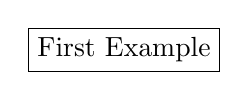
\begin{tikzpicture}
 \node[draw]{First Example};
\end{tikzpicture}}	
\rput(12,0){\fbox{%
  Second example}}	
\end{tkzexample}

\vspace{12pt}


"(x,y)" is the position where "stuff" will be placed."Refpoint" gives the reference point of stuff (text or picture and so on).

\begin{tkzexample}[latex=5cm]
baseline->
\rput{45}(12,0){\fbox{Stuff}}	
\end{tkzexample}



The specifications of the \Verb|\rput| command is:
\begin{docspec}
\large
 \color{blue!50!black} \doccmd{rput[\docopt{options}]\{\docopt{rotation}\}(\docarg{refpoint})\{\docarg{stuff}\}}
\end{docspec}

The first mandatory argument (in parenthesis) is the coordinate pair of the point where the stuff is placed.\\
The second mandatory argument (in curly braces) is the stuff to place.\\ 

The first optional argument is given in brackets and it determines the position of the bounding box of the object to place with respect to the "refpoint" (in parenthesis). The admissible values are mc, t, tl, tr, b, bl, br and B, Br, Bl. The default is mc meaning middle – center , t is for top of the box, b for bottom and B for baseline; r and l are for right and left. We can call these points, the anchors.\\

The second optional argument is given in curly braces. It is a number that stands for the rotation angle.


What is the  baseline ?

As you probably know \TeX\ puts all its objects in boxes. A box has a baseline that determines height and depth.
\begin{marginfigure}
  \centering
    \includegraphics[width=1\textwidth]{baseline.png}
  \caption{The baseline}
  \label{fig:baseline}
\end{marginfigure}

 \TeX\ uses the baselines for fixing together the boxes to others. A box has ten anchors:\\
 -  mc the middle-center, the center point,\\
 -  bl br tl tr are the 4 corners  (for bottom left and bottom right top left and top right),\\   
 -  two anchors Bl and Br (Baseline left and right),\\ 
 -  the vertical line through the middle-center defines three other points t, B and b on the top line, the baseline and the bottom line.

\doccmd{rput} command will place the box defined by using the reference point and placing on this, one of the ten anchors box.
\begin{marginfigure}
  \centering
    \includegraphics[width=1\textwidth]{TeX_box.png}
  \caption{Anchors of a box}
  \label{}
\end{marginfigure}

\newpage
\subsection{Arguments and  options} % (fold)
\label{sub:the_options}

Available anchors:

\begin{table}[h]\index{tikzrput!options}
{ \small   \begin{tabular}{lll}
      \toprule
 name & default  &  definition \\
\midrule
\docoption{mc}{rput} & \{ \}  & middle center mc or empty\\
\docoption{B}{rput}  & \{ \}  & baseline center\\
\docoption{Bl}{rput} & \{ \}  & baseline left  \\
\docoption{Br}{rput} & \{ \}  & baseline right \\
\docoption{t}{rput}  & \{ \}  & top center  \\
\docoption{tl}{rput} & \{ \}  & top left  \\
\docoption{tr}{rput} & \{ \}  & top right\\
\docoption{b}{rput}  & \{ \}  & bottom center \\
\docoption{bl}{rput} & \{ \}  & bottom left\\
\docoption{br}{rput} & \{ \}  & bottom right \\ 
\midrule
\docoption{rotation}{rput} & 0  & angle of rotation around ref point \\ 
\bottomrule
\end{tabular} }
\caption{List of  options for the pgfornament macro.} 
  \label{tab:pgfornament-options}
\end{table} 

 The angle of \docopt{rotation} is expressed in degrees...\\
 The \docarg{refpoint} is defined by two coordinates \Verb|(x,y)|. 
% subsection the_options (end) 


\newpage

\section{Examples} % (fold)
\label{sec:examples}
\subsection{ex 1 Ornaments patterns} % (fold)
\label{sub:ex_1}

  
\begin{tkzexample}[code only,small]
\hspace{1cm}%
\rput[r](-3pt,3pt){\pgfornament[scale=.2]{72}}
  		{Ornaments patterns}%
\rput[l](3pt,3pt){\large\pgfornament[scale=.2]{73}}
\end{tkzexample} 
\begin{marginfigure}
\hspace{1cm}\rput[r](-3pt,3pt)
 {\pgfornament[scale=.2]{72}}
  {Ornaments patterns}%
  \rput[l](3pt,3pt)
  {\large\pgfornament[scale=.2]{73}}
\end{marginfigure}
% subsection ex_1 (end)
% section examples (end)

\subsection{ex 2  Ornaments} % (fold)
\label{sub:ex_2_ornaments}

\begin{tkzexample}[code only,small]
\documentclass{scrartcl} 
\usepackage[utf8]{inputenc} 
\usepackage[T1]{fontenc} 
\usepackage[dvipsnames]{xcolor}
\usepackage{tikzrput}
\usepackage{pgfornament} 
\begin{document}  
\tikzset{pgfornamentstyle/.style={%
		draw = Periwinkle,
        fill = SpringGreen}}
\unitlength=1cm
\begin{picture}(10,10)%
  \color{blue}%
   \put(0,0){\framebox(10,10){%
   \rput[tl](-3,5){\pgfornament[width=6cm]{71}}%
   \rput[bl](-3,-5){\pgfornament[width=6cm,
   								symmetry=h]{71}}%
   \rput[tl](-5,5){\pgfornament[width=2cm]{63}}%
   \rput[tr](5,5){\pgfornament[width=2cm,
   							   symmetry=v]{63}}%
   \rput[bl](-5,-5){\pgfornament[width=2cm,
   							     symmetry=h]{63}}%
   \rput[br](5,-5){\pgfornament[width=2cm,
   								symmetry=c]{63}}%
   \rput[bl]{-90}(-5,3){\pgfornament[width=6cm]{46}}%
   \rput[bl]{90}(5,-3){\pgfornament[width=6cm]{46}}%
   \rput(0,0){\Huge \color{MidnightBlue} Ornaments}%
   \rput[t](0,-0.5){\pgfornament[width=5cm]{75}}%
   \rput[b](0,0.5){\pgfornament[width=5cm]{69}}%
   \rput[tr]{-30}(-1,2.5){\pgfornament[width=2cm]{57}}%
   \rput[tl]{30}(1,2.5){\pgfornament[width=2cm,symmetry=v]{57}}}}% 
\end{picture} 
\end{document} 
\end{tkzexample}
\begin{marginfigure}
	  \centering
	    \includegraphics[width=1\textwidth]{ornaments.png}
	  \caption{caption}
	  \label{fig:ornaments}
\end{marginfigure}
% subsection ex_2_blue_ornament (end)

\subsection{ex3 Picture} % (fold)
\label{sub:ex3_picture}
\begin{tkzexample}[code only,small]
\documentclass{article}
\usepackage[utf8]{inputenc} 
\usepackage[T1]{fontenc} 
\usepackage[dvipsnames]{xcolor}
\usepackage{pict2e,tikzrput} 
\usepackage[calc]{picture}
\usepackage[]{fourier} 
\begin{document}

\setlength{\parindent}{0pt} 
\setlength{\unitlength}{1cm}
  \begin{picture}(3,3)
    \put(0,0){\framebox(3,3){}}%
    \color{blue}%
    \thicklines
    \put(0,0){\line(1,1){3}}
    \color{MidnightBlue}% 
    \rput[b]{45}(2,2){\large \textbf{line}} 
  \end{picture}%  

\end{document}
\end{tkzexample}
\begin{marginfigure}
\centering
   \setlength{\parindent}{0pt} 
   \setlength{\unitlength}{1cm}
     \begin{picture}(3,3)
       \put(0,0){\framebox(3,3){}}%
       \color{blue}%
       \thicklines
       \put(0,0){\line(1,1){3}}
       \color{MidnightBlue}% 
       \rput[b]{45}(2,2){\large \textbf{line}} 
     \end{picture}% 
   	  \caption{with picture}
   	  \label{fig:picture}
\end{marginfigure}
% subsection ex3_picture (end)

\subsection{ex 4 Tikzpicture} % (fold)
\label{sub:ex_4_tikzpicture}
\begin{tkzexample}[code only,small]
\documentclass{article}
\usepackage[utf8]{inputenc} 
\usepackage[T1]{fontenc} 
\usepackage[dvipsnames]{xcolor}
\usepackage{pict2e,tikzrput} 
\usepackage[calc]{picture}
\usepackage{fourier} 
\begin{document}

\hrule
baseline%
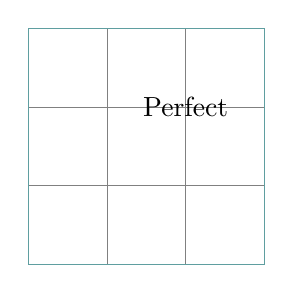
\begin{tikzpicture}[baseline=(current bounding box.south west)] 
 \draw[help lines] (0,0) grid (3,3) ;
 \draw[use as bounding box,color=CadetBlue](0,0)rectangle(3,3);    
 \rput (2,2){Perfect}% 
\end{tikzpicture}%
baseline% 

\end{document}	
\end{tkzexample}
\begin{marginfigure}
\hrule
baseline%
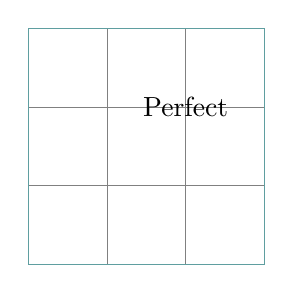
\begin{tikzpicture}[baseline=(current bounding box.south west)] 
 \draw[help lines] (0,0) grid (3,3) ;
 \draw[use as bounding box,color=CadetBlue] (0,0) rectangle (3,3) ;    
 \rput (2,2){Perfect}% 
\end{tikzpicture}%
baseline% 
   	  \caption{with tikzpicture}
   	  \label{fig:tikzpicture}
\end{marginfigure}
% subsection ex_4_tikzpicture (end)
\newpage
\subsection{ex 5 From pstricks doc} % (fold)
\label{sub:ex_5_from_pstricks_doc}
\begin{marginfigure}	
	 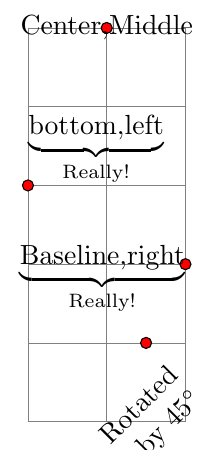
\begin{tikzpicture}[baseline=(current bounding box.north)] 
	      \draw[help lines] (-1,0) grid (1,5) ; 
	 \foreach \x/\y in {0/5,-1/3,1/2,0.5/1} {%
	      \rput(\x,\y ){\tikz\draw[fill=red] circle(2pt);};} 
	\rput(0,5){Center,Middle}
	\rput[bl](-1,3){$\underbrace{\text{bottom,left}}_{\text{Really!}}$}
	\rput[Br](1,2){$\underbrace{\text{Baseline,right}}_{\text{Really!}}$}
	\rput[tr]{45}(0.5,1)
	{\parbox{5cm}{\flushright Rotated\\
	by $45^{\circ}$}}
	\end{tikzpicture}  
   	  \caption{from pstricks}
   	  \label{fig:from pstricks}
\end{marginfigure}
	As we have already seen, the \Verb+{\rput}+ macro can be used to place objects.
	The second mandatory argument (in curly braces) is the stuff to place the first
	mandatory argument (in parenthesis) is the coordinate pair of the point where
	the stuff is placed.
	Now we turn to the optional arguments of the \Verb+{\rput}+ macro.
	The first one is given in brackets. It determines the justification of the
	bounding box of the object to place with respect to the point given in paren-
	thesis. The admissible values are the same as the values for the option origin
	of the \verb+{\includegraphics}+ macro. For an instance \Verb+{[br]}+ for bottom-right.
	The default is mc meaning middle - center.
	The second optional argument is given in curly braces just before the left
	parenthesis. It is a number that stands for the rotation angle as illustrated in
	the last instance of the \Verb+{\rput}+ macro on the slide.
	The two optional arguments make \Verb+{\rput}+ more 
	exible than the \Verb+{\put}+ macro
	of the picture environment. 
	\rput[b](-2,0){%
	
\begin{tikzpicture}[%
		every node/.style={inner sep=0pt}]
	  \tikzset{image/.style={circle,
	                         fill=red,
	                         minimum size = 4pt,
	                         inner sep    = 0pt,
	                         outer sep    = 1pt}
	                         }
	\node[inner sep = 1cm] (wrapper){\tikz
	\node(image) {\pgfornament[scale=1.5,opacity=0.2]{1}};};
	\end{tikzpicture}}

\begin{tkzexample}[code only,small]
	\rput[b](-2,0){%
	
\begin{tikzpicture}[%
		every node/.style={inner sep=0pt}]
	  \tikzset{image/.style={circle,
	                         fill=red,
	                         minimum size = 4pt,
	                         inner sep    = 0pt,
	                         outer sep    = 1pt}
	                         }
	\node[inner sep = 1cm] (wrapper){\tikz
	\node(image) {\pgfornament[scale=1.5,opacity=0.2]{1}};};
	\end{tikzpicture}}	
\end{tkzexample}	
% subsection ex_5_from_pstricks_doc (end)

\subsection{ex 6 From pstricks again} % (fold)
\label{sub:ex_6_from_pstricks_again}
\def\myEye{
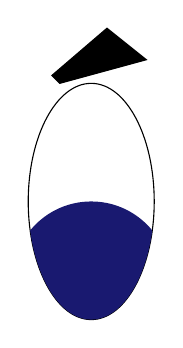
\begin{tikzpicture}  
   \filldraw (-0.4,1.5)--(0.7,1.8)--(0.2,2.2)--(-0.5,1.6)--cycle;   
   \draw [clip] (0,0) circle [x radius=.8cm, y radius=1.5cm]; 
   \fill[MidnightBlue] (0,-1) circle [radius=1cm];
\end{tikzpicture}        
}
\begin{marginfigure}	
\rput{30}(2,-6){Tu as de beaux yeux !}
\rput(3,-3){\myEye}
\rput(1,-3){\reflectbox{\myEye}}
   	  \caption{from pstricks again}
   	  \label{fig:from pstricks again}
\end{marginfigure}
\begin{tkzexample}[code only,small]
\documentclass{scrartcl}
\PassOptionsToPackage{dvipsnames,svgnames}{xcolor}  
\usepackage{tikzrput}
\begin{document}

\rput{30}(7,-5){Tu as de beaux yeux !}
\rput(8,-2){\myEye}
\rput(6,-2){\reflectbox{\myEye}}
 \end{document} 	
\end{tkzexample}
\def\myEye{
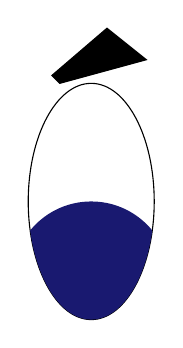
\begin{tikzpicture}  
   \filldraw (-0.4,1.5)--(0.7,1.8)--(0.2,2.2)--(-0.5,1.6)--cycle;   
   \draw [clip] (0,0) circle [x radius=.8cm, y radius=1.5cm]; 
    \fill[MidnightBlue] (0,-1) circle [radius=1cm];
\end{tikzpicture}        
}


% subsection ex_6_from_pstricks_again (end)

\subsection{ex 7 Ancres} % (fold)
\label{sub:ex_7_ancres}
Utilisation des ancres

\begin{tkzexample}[code only,small]
\documentclass{scrartcl}
\PassOptionsToPackage{dvipsnames,svgnames}{xcolor}  
\usepackage{tikzrput}
\begin{document}
-->\rput[]   (5,0){\tikz \draw[blue]  (0,0) rectangle +(1,2);}
   \rput[tl] (5,0){\tikz \draw[red]   (0,0) rectangle +(1,2);}
   \rput[br] (5,0){\tikz \draw[green] (0,0) rectangle +(1,2);}
   \rput[Bl] (5,0){\tikz \draw[orange](0,0) rectangle +(1,2);}
\end{document}
\end{tkzexample}
\begin{marginfigure}	
-->\rput[] (5,0)  {\tikz \draw[blue]  (0,0) rectangle +(1,2);}
   \rput[tl] (5,0){\tikz \draw[red]   (0,0) rectangle +(1,2);}
   \rput[br] (5,0){\tikz \draw[green] (0,0) rectangle +(1,2);}
   \rput[Bl] (5,0){\tikz \draw[orange](0,0) rectangle +(1,2);}
   	  \caption{ancres}
   	  \label{fig:ancres}
\end{marginfigure}

% subsection ex_7_ancres (end)

 
\newpage

\printindex 

\end{document}  





    